\documentclass[aspectratio=43,10pt]{beamer}

\usetheme{Warsaw}
\usefonttheme{professionalfonts}
\usepackage[T1]{fontenc}
\usepackage[utf8]{inputenc}
\usepackage{newtxtext,newtxmath}
\usepackage{graphicx}
\usepackage{booktabs}
\usepackage{array}
\usepackage{colortbl}
\usepackage{ragged2e}
\usepackage{amsmath}
\usepackage{etoolbox}
\newcommand{\currentsliderefs}{}
\newcommand{\currentsymbols}{}
\newsavebox{\slideannotationsbox}
\newcommand{\sliderefs}[1]{\gdef\currentsliderefs{#1}}
\BeforeBeginEnvironment{frame}{\gdef\currentsliderefs{}\gdef\currentsymbols{}}

\definecolor{inatelblue}{HTML}{045FB4}
\definecolor{inatelnavy}{HTML}{17365D}
\setbeamercolor{structure}{fg=inatelblue}
\setbeamercolor{palette primary}{bg=inatelblue,fg=white}
\setbeamercolor{palette secondary}{bg=inatelnavy,fg=white}
\setbeamercolor{palette tertiary}{bg=inatelblue,fg=white}
\setbeamercolor{palette quaternary}{bg=inatelnavy,fg=white}
\setbeamercolor{frametitle}{bg=inatelblue,fg=white}
\setbeamercolor{title}{fg=white}
\setbeamercolor{block title}{bg=inatelblue,fg=white}
\setbeamercolor{block body}{bg=blue!4,fg=black}
\setbeamercolor{footline}{bg=black,fg=white}
\setbeamerfont{author}{size=\Large}
\setbeamerfont{institute}{size=\large}
\setbeamerfont{date}{size=\large}
\setbeamertemplate{navigation symbols}{}
\setbeamertemplate{caption}[numbered]
\setbeamerfont{caption}{size=\scriptsize,series=\mdseries}
\setbeamerfont{caption name}{size=\scriptsize,series=\bfseries}
\setbeamercolor{caption}{fg=black}
\setbeamercolor{caption name}{fg=black}
\setlength{\abovecaptionskip}{2pt}
\setlength{\belowcaptionskip}{2pt}
\newcommand{\slideannotations}{%
  \ifx\currentsymbols\empty\else
    \begin{beamercolorbox}[wd=\paperwidth,leftskip=10pt,rightskip=10pt]{normal text}%
      \usebeamercolor[fg]{normal text}\fontsize{6}{7}\selectfont\raggedright\leftskip=10pt\rightskip=10pt plus 1fil
      \textbf{Symbols:} \currentsymbols\par
    \end{beamercolorbox}%
  \fi
  \ifx\currentsliderefs\empty\else
    \nointerlineskip
    \begin{beamercolorbox}[wd=\paperwidth,leftskip=10pt,rightskip=10pt]{normal text}%
      \usebeamercolor[fg]{normal text}\fontsize{5}{6}\selectfont\raggedright\leftskip=10pt\rightskip=10pt plus 1fil\currentsliderefs\par
    \end{beamercolorbox}%
  \fi
  \vskip2pt}
\newcommand{\symbolnote}[1]{%
  \gdef\currentsymbols{#1}%
  \par\setbox\slideannotationsbox=\vbox{\slideannotations}%
  \vspace*{\dimexpr\ht\slideannotationsbox+\dp\slideannotationsbox\relax}}
\newcommand{\tablerowseparator}{\midrule[.25pt]}
\setbeamertemplate{footline}{%
  \vbox to 0pt{\vss\slideannotations}%
  \nointerlineskip
  \leavevmode\hbox{%
  \begin{beamercolorbox}[wd=.86\paperwidth,ht=2.6ex,dp=1.1ex,leftskip=1em]{footline}%
    \insertshorttitle
  \end{beamercolorbox}%
  \begin{beamercolorbox}[wd=.14\paperwidth,ht=2.6ex,dp=1.1ex,center]{footline}%
    \insertframenumber
  \end{beamercolorbox}}}
\setbeamertemplate{headline}{%
  \leavevmode\hbox{%
  \begin{beamercolorbox}[wd=.82\paperwidth,ht=2.3ex,dp=.9ex,leftskip=1em]{palette primary}\insertsectionhead\end{beamercolorbox}%
  \begin{beamercolorbox}[wd=.18\paperwidth,ht=2.3ex,dp=.9ex,center]{palette secondary}\textbf{Inatel}\end{beamercolorbox}}}

\usepackage{tikz}
\setbeameroption{hide notes}
\newcommand{\fig}[2]{\begin{center}\includegraphics[width=.92\linewidth,height=#2\textheight,keepaspectratio]{assets/#1}\end{center}}
\newcommand{\takeaway}[1]{\begin{beamercolorbox}[rounded=true,sep=.6ex]{block body}\textbf{Takeaway:} #1\end{beamercolorbox}}

\title[Air-only inverse design]{Training forward surrogates for air-only gold nanostructure inverse design}
\author[M. F. Silva]{Matheus Ferreira Silva}
\institute[Inatel]{National Institute of Telecommunications (Inatel)\\[.6ex]
Supervisor: Prof. Dr. Felipe Augusto Pereira de Figueiredo\\
Co-supervisor: Prof. Dr. Rausley Adriano Amaral de Souza}
\date{November 2026}

% Timed main sequence: 580 seconds (9 min 40 s), 14 main slides.
\begin{document}

\section{Overview}
\begin{frame}{Problem and workflow}
  \fig{pipeline.pdf}{.40}
  \begin{itemize}
    \item Request: target absorption over a wavelength band.
    \item A trained surrogate guides gradient-based geometry search.
    \item HFSS supplies the physical check.
  \end{itemize}
  \vfill
  \takeaway{The workflow connects received HFSS data to an auditable physical verification.}
  \note{0:40. Explicar cada etapa da esquerda para a direita.}
\end{frame}

\section{Dataset}
\begin{frame}{Received air-only dataset}
  \fig{geometries.pdf}{.57}
  {\centering\scriptsize Twelve received geometry families. Counts are unique geometries after duplicate grouping.\par}
  \vfill
  \takeaway{Keeping duplicate geometries together prevents an inflated test metric.}
  \note{0:40. São 2.000 espectros, 1.926 geometrias únicas, todas em ar.}
\end{frame}

\begin{frame}{Two uses of the same dataset}
  \begin{columns}[c]
    \column{.54\linewidth}\centering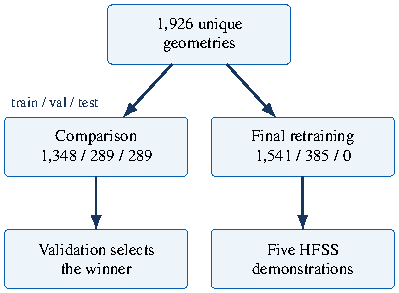
\includegraphics[width=\linewidth,height=.56\textheight,keepaspectratio]{assets/splits.pdf}
    \column{.44\linewidth}\small
    \textbf{Model input}
    \begin{itemize}\item family ID\item seven native parameters\item family mask\end{itemize}
    \textbf{Model output}
    \begin{itemize}\item 401 wavelengths\item $T,R,A$ with a softmax at each wavelength\end{itemize}
  \end{columns}
  \vfill
  \takeaway{Held-out metrics and physical HFSS results belong to different model sets.}
  \symbolnote{$T,R,A$: transmitted, reflected, and absorbed power fractions. Splits are train / validation / test geometry counts.}
  \note{0:35. Destacar que os modelos finais não têm conjunto de teste.}
\end{frame}

\section{Training}
\begin{frame}{Surrogate model and training objective}
  \fig{model.pdf}{.36}
  {\centering\small Training: 300 epoch cap, patience 30, batch size 64. Atomic model, optimizer, and random-state recovery enables resumption.\par}
  \vfill
  \takeaway{The loss targets absorption directly, including its worst-case error per spectrum, with $T/R/A$ as an auxiliary term.}
  \symbolnote{MLP: multilayer perceptron. $\lambda$: wavelength. The softmax enforces $T+R+A=1$ but does not prove physical realizability.}
  \note{0:40. Explicar entradas, MLP e softmax por comprimento de onda.}
\end{frame}

\begin{frame}{Four independent comparison cases}
  \vspace{0pt}
  {\small\centering
  \begin{tabular}{lll}
    \toprule Case & selection & selected topology\\\midrule
    Baseline & fixed & residual, $256\times3$, dropout 0.1\\
    Optuna & 100 candidates & plain, $256\times3$, dropout 0\\
    Ray & 100 early-stopped candidates & plain, $256\times3$, dropout 0\\
    AutoKeras & AutoModel then PyTorch export & plain, $128\times3$\\\bottomrule
  \end{tabular}\par}
  \vspace{1ex}
  \begin{block}{Search space}
    \centering Plain or residual trunk, width 128/256/512, depth 2--5, dropout 0/0.1/0.2.\par
    \scriptsize Optuna: 54 completed and 46 pruned candidates. AutoKeras: 57 completed.
  \end{block}
  \vfill
  \takeaway{Optuna and Ray selected the same topology, but remain independent comparison cases.}
  \note{0:45. Mostrar que a busca seleciona apenas por validação.}
\end{frame}

\begin{frame}{Training and search results}
  \fig{training.pdf}{.29}\vspace{-1.5ex}
  {\centering\scriptsize Training and validation histories.\par}
  \fig{search.pdf}{.26}\vspace{-1.5ex}
  {\centering\scriptsize Best validation loss by search trial.\par}
  \vfill
  \takeaway{The searched cases improve validation loss relative to the fixed baseline.}
  \note{0:35. Não discutir variações pequenas, focar na tendência de validação.}
\end{frame}

\begin{frame}{Error on 289 held-out geometries}
  \vspace{1.5ex}
  {\small\centering
  \begin{tabular}{lrrr}
    \toprule Case & MAE (pp) & mean max (pp) & P95 max (pp)\\\midrule
    AutoKeras&1.45&6.52&13.02\\ Ray&1.50&6.87&13.28\\ Optuna&1.55&6.92&12.95\\ Baseline&1.95&8.48&15.90\\\bottomrule
  \end{tabular}\par}
  \fig{families_error.pdf}{.33}\vspace{-1.5ex}
  {\centering\scriptsize Absorption MAE per geometry family.\par}
  \vfill
  \takeaway{Absorption MAE spans 1.45--1.95 percentage points across the four cases.}
  \symbolnote{MAE: mean absolute absorption error. mean max and P95 max: mean and 95th percentile of the largest absorption error per spectrum. pp: percentage points.}
  \note{0:40. Métrica em teste se aplica somente à comparação 1348/289/289.}
\end{frame}

\begin{frame}{Effect of training-set size}
  \fig{learning_curve.pdf}{.50}
  {\centering\small\textit{Nested family-stratified subsets of the fixed 1,348 training geometries, three seeds per point. Error bars: sample SD over three seeds. Topologies selected with 1,348 rows are held fixed.}\par}
  \vfill
  \takeaway{Error drops strongly up to 674--1,011 geometries. The last step is not uniformly better. Silica data remain pending.}
  \note{0:45. 45 treinos concluídos. A queda é forte nos primeiros tamanhos, mas o ganho final não é monotônico em todos os modelos. Barras indicam desvio entre três sementes. A topologia foi selecionada com 1348 geometrias.}
\end{frame}

\begin{frame}{Held-out spectra selected by a fixed rule}
  \fig{held_out.pdf}{.66}
  \vfill
  \takeaway{Best, median, and P95 examples are fixed quantiles of baseline maximum absorption error, not hand-picked spectra.}
  \note{0:45. Identificadores: G1138 F08, G1257 F09 e G0234 F03. Mostrar os zooms.}
\end{frame}

\section{Inference}
\begin{frame}{Inference under geometry constraints}
  \fig{inference.pdf}{.40}
  \begin{center}$\displaystyle\min_{\theta}\;\max_{\lambda\in[\lambda_1,\lambda_2]}\bigl|\hat A(\lambda;\theta)-A_\star\bigr|$, then wavelength-weighted mean error.\end{center}
  \vfill
  \takeaway{Candidates remain inside training bounds and local trust regions, with positive ring holes.}
  \symbolnote{$\lambda_1,\lambda_2$: band edges. $A_\star$: target absorption. $\hat A$: surrogate absorption. $\theta$: native geometry parameters of one family.}
  \note{0:45. Explicar os 12 por 8 inícios e os 500 passos.}
\end{frame}

\begin{frame}{Five narrow-band HFSS demonstrations}
  \fig{hfss_errors.pdf}{.32}
  {\centering\scriptsize\setlength{\tabcolsep}{4pt}
  \begin{tabular}{lccccccc}
    \toprule
    Worst HFSS error (pp) & \shortstack{Ex.\,1\\500--510\\40\%} & \shortstack{Ex.\,2\\600--620\\30\%} & \shortstack{Ex.\,3\\750--780\\25\%} & \shortstack{Ex.\,4\\1000--1040\\20\%} & \shortstack{Ex.\,5\\1250--1300\\15\%} & Mean & $\le5$ pp\\
    \midrule
    Baseline&0.23&1.05&12.98&2.99&1.90&3.83&4/5\\
    Optuna = Ray&0.14&3.08&3.22&0.61&2.94&2.00&5/5\\
    AutoKeras&0.30&2.49&11.44&2.61&0.63&3.49&4/5\\
    \bottomrule
  \end{tabular}\par}
  \vfill
  \takeaway{These five dataset-supported demonstrations are not a blind generalization test.}
  \symbolnote{Ex.: request, with band in nm and target absorption. Error: largest in-band difference between HFSS absorption and target.}
  \note{0:50. Optuna e Ray são iguais por terem tensores idênticos.}
\end{frame}

\begin{frame}{HFSS spectra include a difficult case}
  \fig{hfss_spectra.pdf}{.58}
  {\centering\small Baseline, example 3: surrogate worst error 0.88 pp, HFSS worst error 12.98 pp.\par}
  \vfill
  \takeaway{Physical verification exposes surrogate optimism even when the predicted target error is small.}
  \note{0:50. Contrastar caso bom com exemplo 3, sem esconder a falha.}
\end{frame}

\begin{frame}{Geometries returned by inference}
  \fig{winners.pdf}{.55}
  {\centering\scriptsize Each geometry is also saved in native nanometres as \texttt{geometry.json}.\par}
  \vfill
  \takeaway{The output is a native-nanometre geometry file ready for a received-template HFSS verification.}
  \note{0:30. Chamar atenção ao exemplo 3: F12 no baseline e AutoKeras, F06 no Optuna e Ray.}
\end{frame}

\section{Conclusions}
\begin{frame}{Conclusions and next steps}
  \begin{columns}[T]
    \column{.49\linewidth}\textbf{Conclusions}
    \begin{itemize}
      \item End-to-end data, training, inference, and HFSS workflow operates.
      \item Held-out absorption MAE is 1.45--1.95 pp.
      \item Most narrow-band demonstrations meet $\pm5$ pp in HFSS.
    \end{itemize}
    \column{.49\linewidth}\textbf{Next steps}
    \begin{itemize}
      \item Receive and prepare 2,000 silica spectra.
      \item Run more HFSS validations.
      \item Reassess data-size learning curves.
    \end{itemize}
  \end{columns}
  \vfill
  \takeaway{The evidence currently supports air-only, narrow-band demonstrations with explicit physical verification.}
  \note{0:40. Fechar em 9:50. Limites: ar, cinco pedidos e otimismo do surrogate.}
\end{frame}

\appendix
\section*{Backup}
\begin{frame}{Backup: HFSS geometry, example 1}\centering
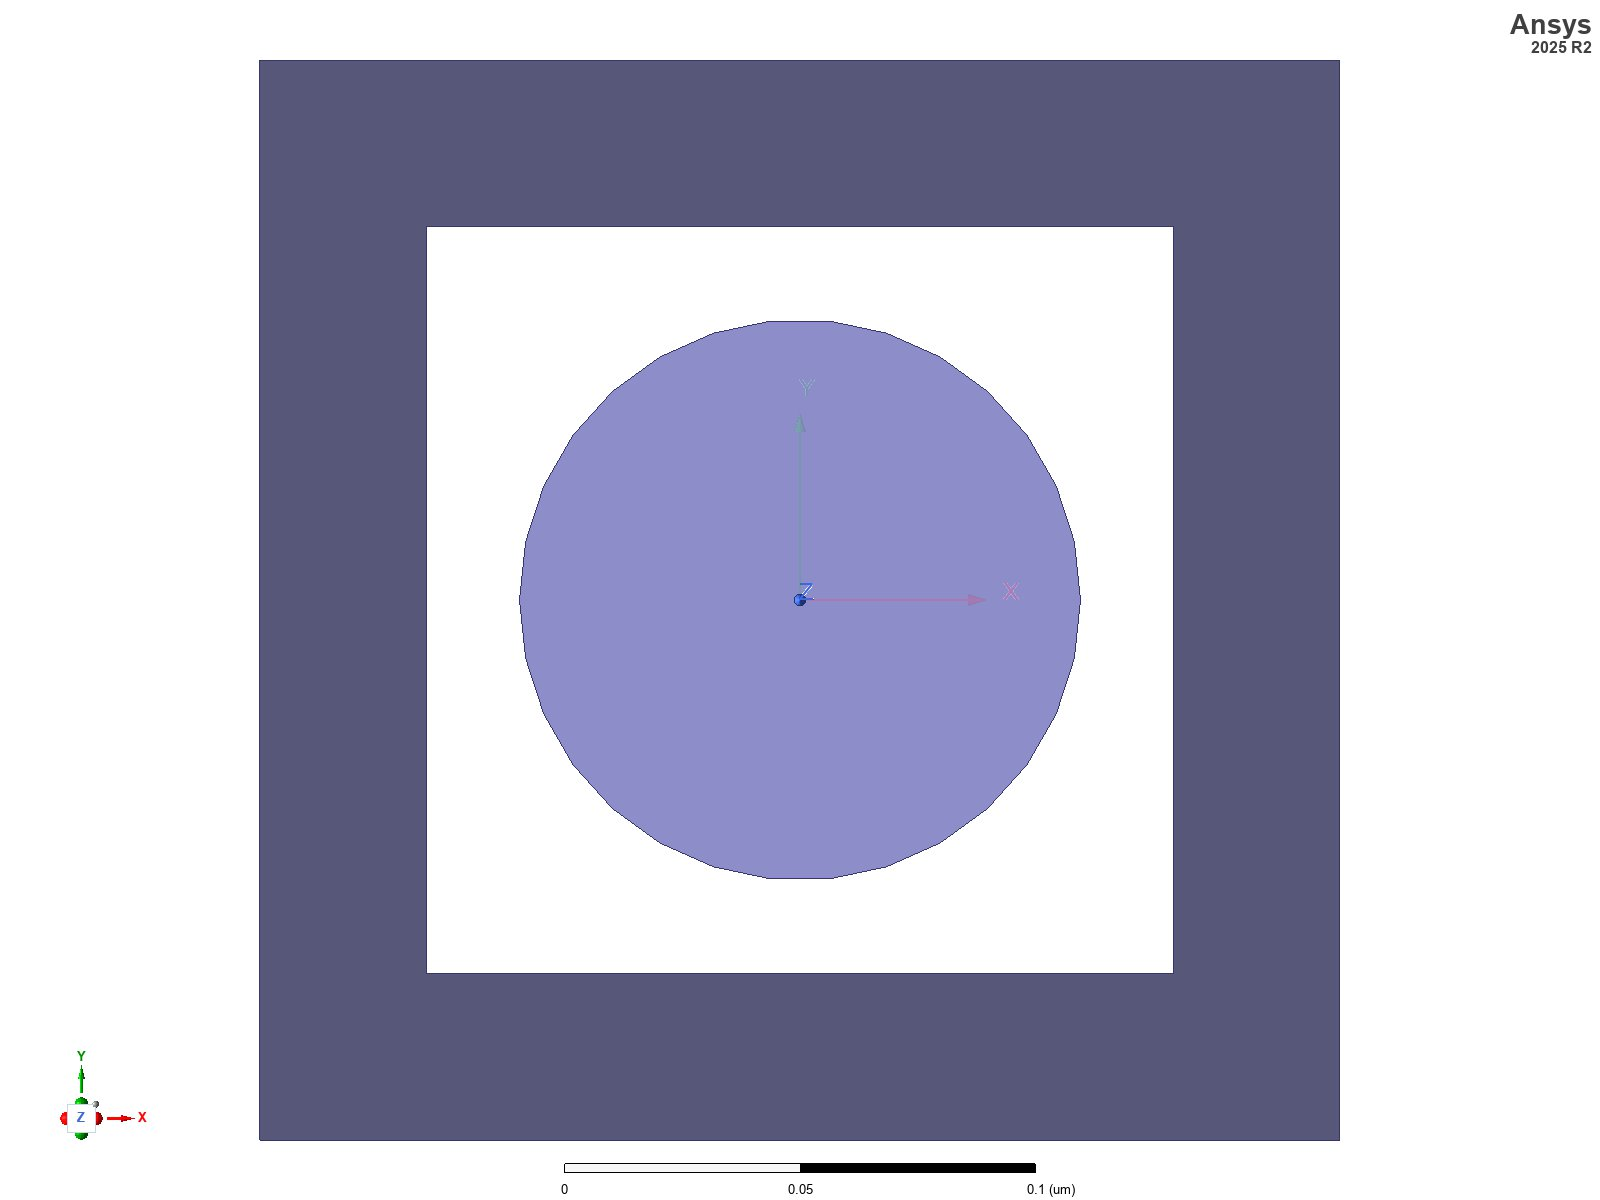
\includegraphics[width=.94\linewidth,height=.72\textheight,keepaspectratio]{assets/hfss/example_01.jpg}\par
{\small Optuna = Ray, F07. Target: 40\% over 500--510 nm.}\par{\scriptsize Top view exported from the verified HFSS project.}\end{frame}

\begin{frame}{Backup: HFSS geometry, example 2}\centering
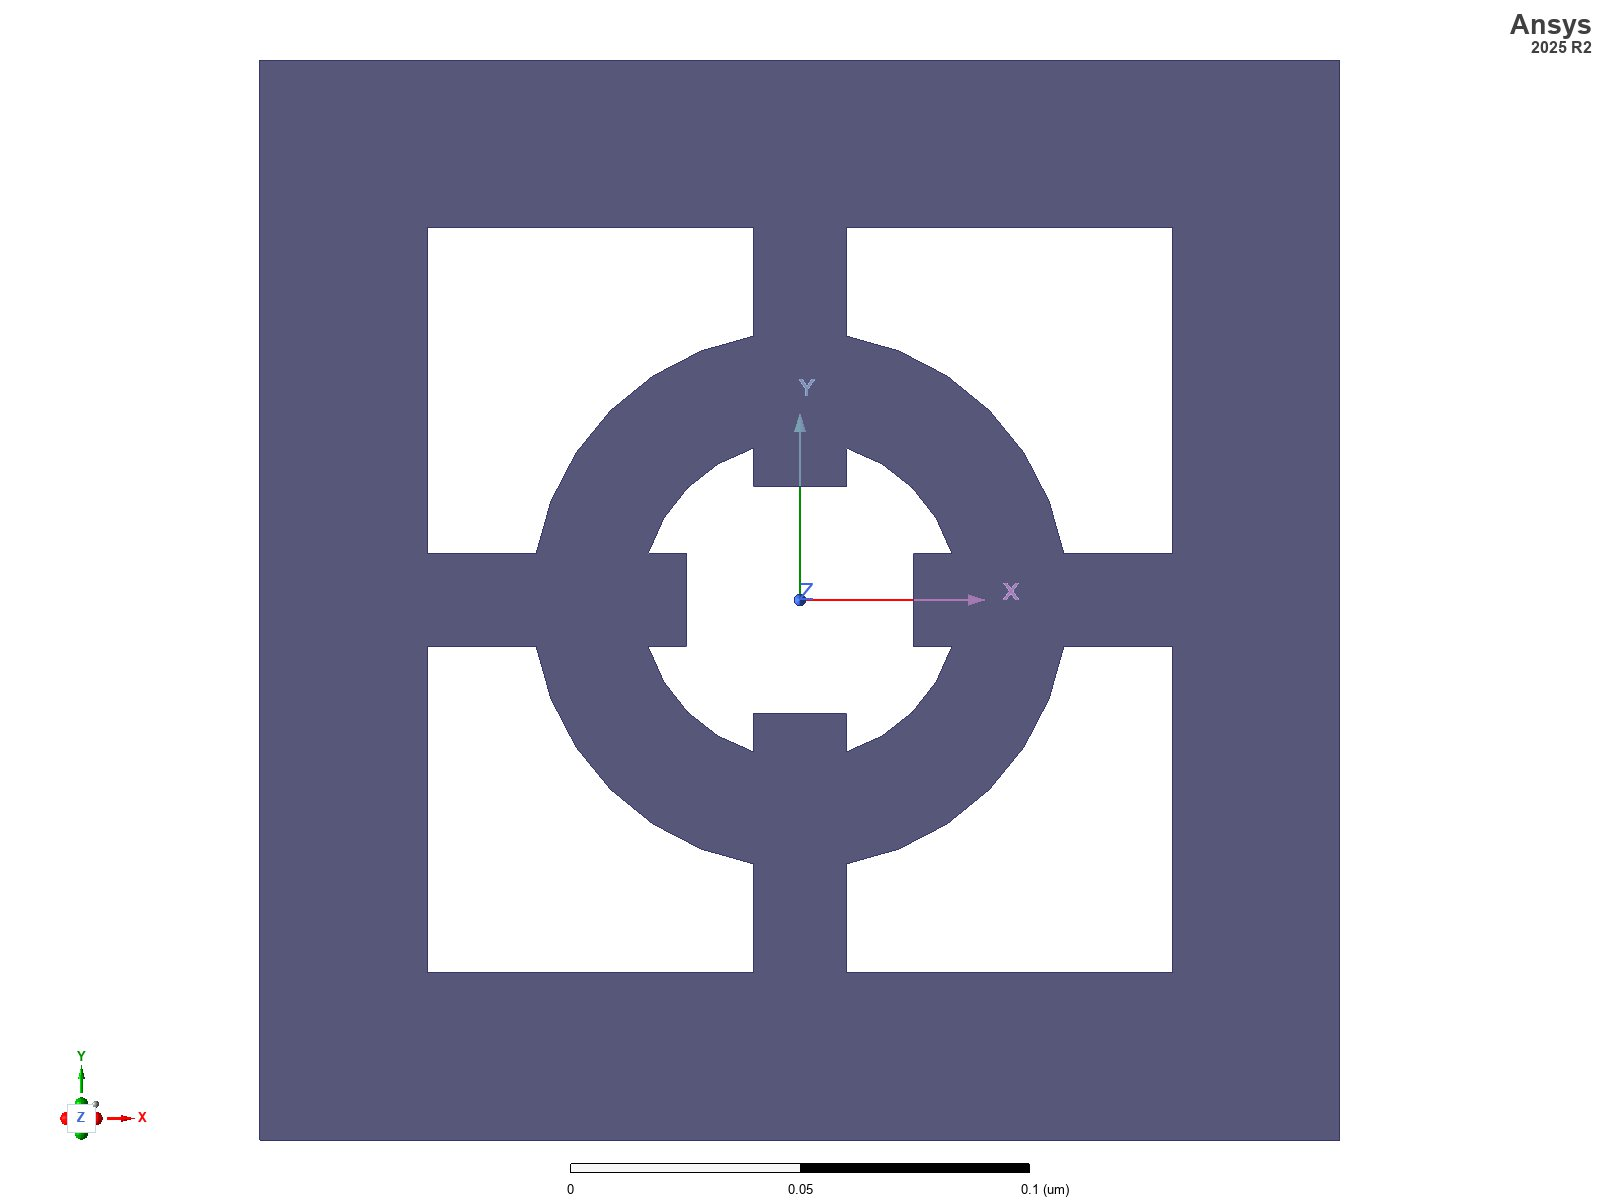
\includegraphics[width=.94\linewidth,height=.72\textheight,keepaspectratio]{assets/hfss/example_02.jpg}\par
{\small Optuna = Ray, F06. Target: 30\% over 600--620 nm.}\par{\scriptsize Top view exported from the verified HFSS project.}\end{frame}

\begin{frame}{Backup: HFSS geometry, example 3}\centering
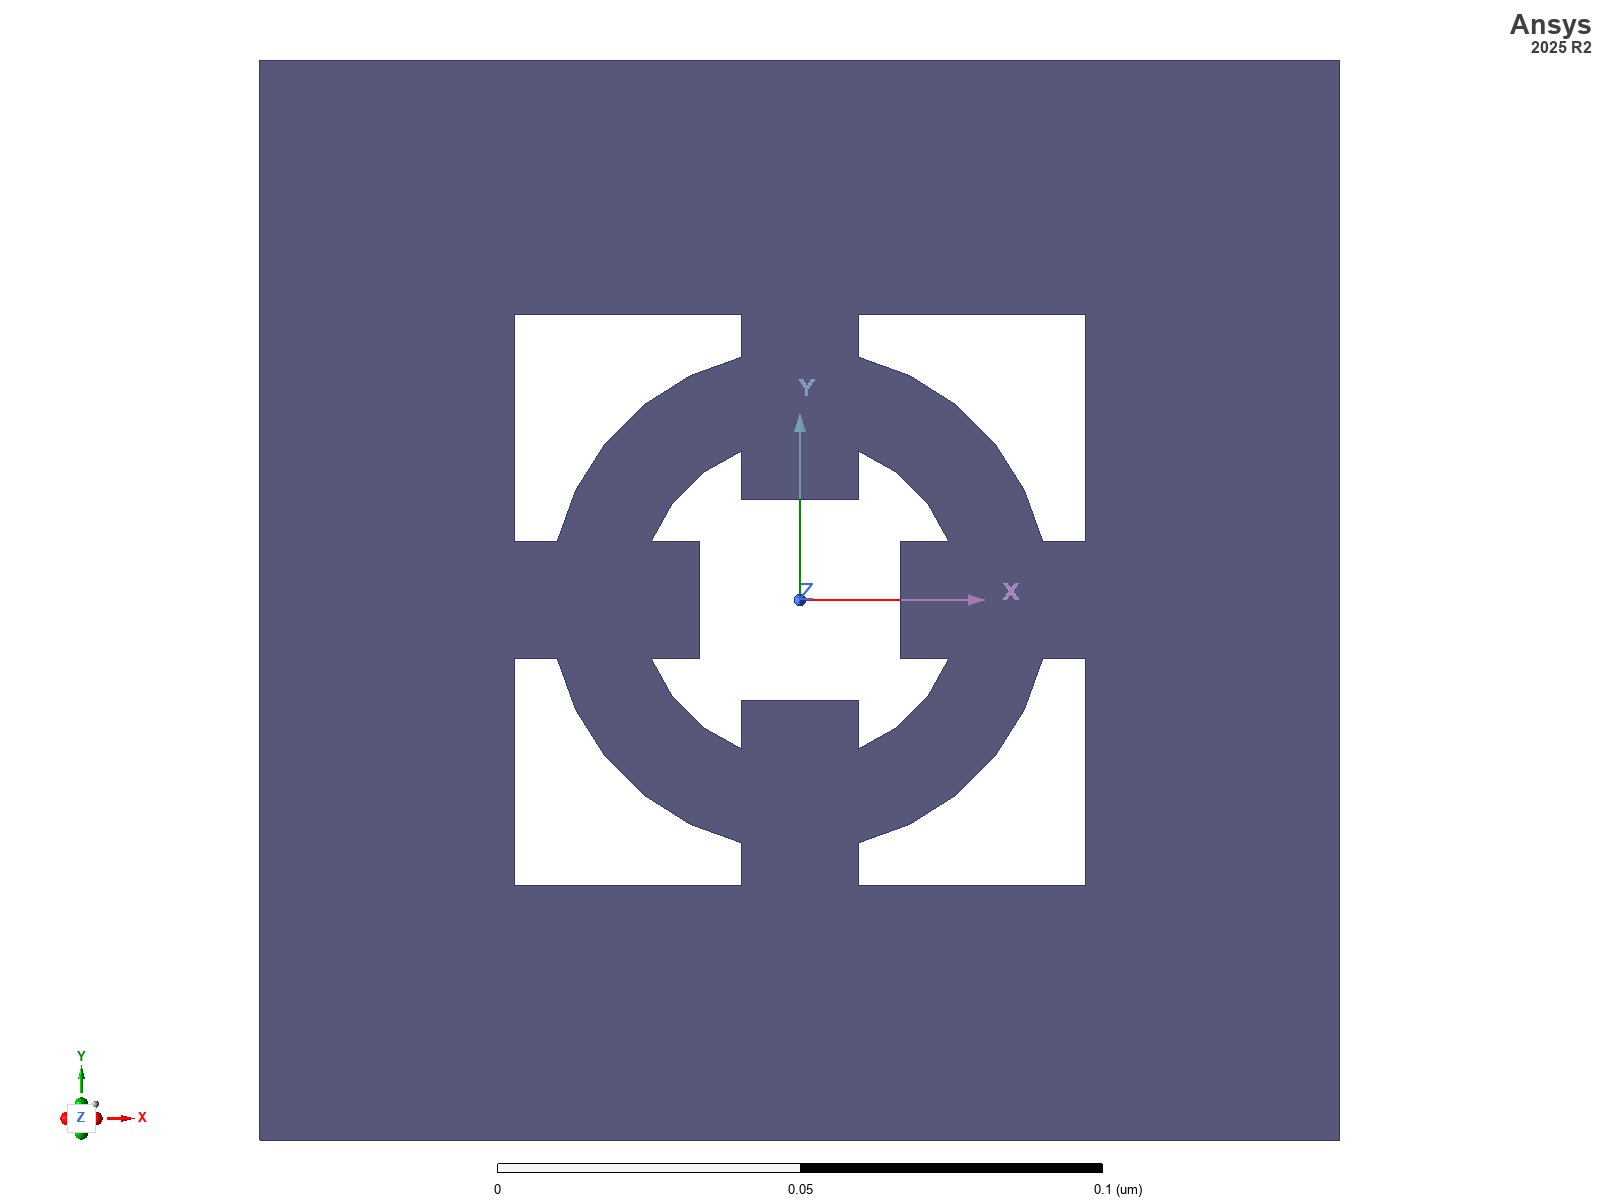
\includegraphics[width=.94\linewidth,height=.72\textheight,keepaspectratio]{assets/hfss/example_03.jpg}\par
{\small Optuna = Ray, F06. Target: 25\% over 750--780 nm.}\par{\scriptsize Top view exported from the verified HFSS project.}\end{frame}

\begin{frame}{Backup: HFSS geometry, example 4}\centering
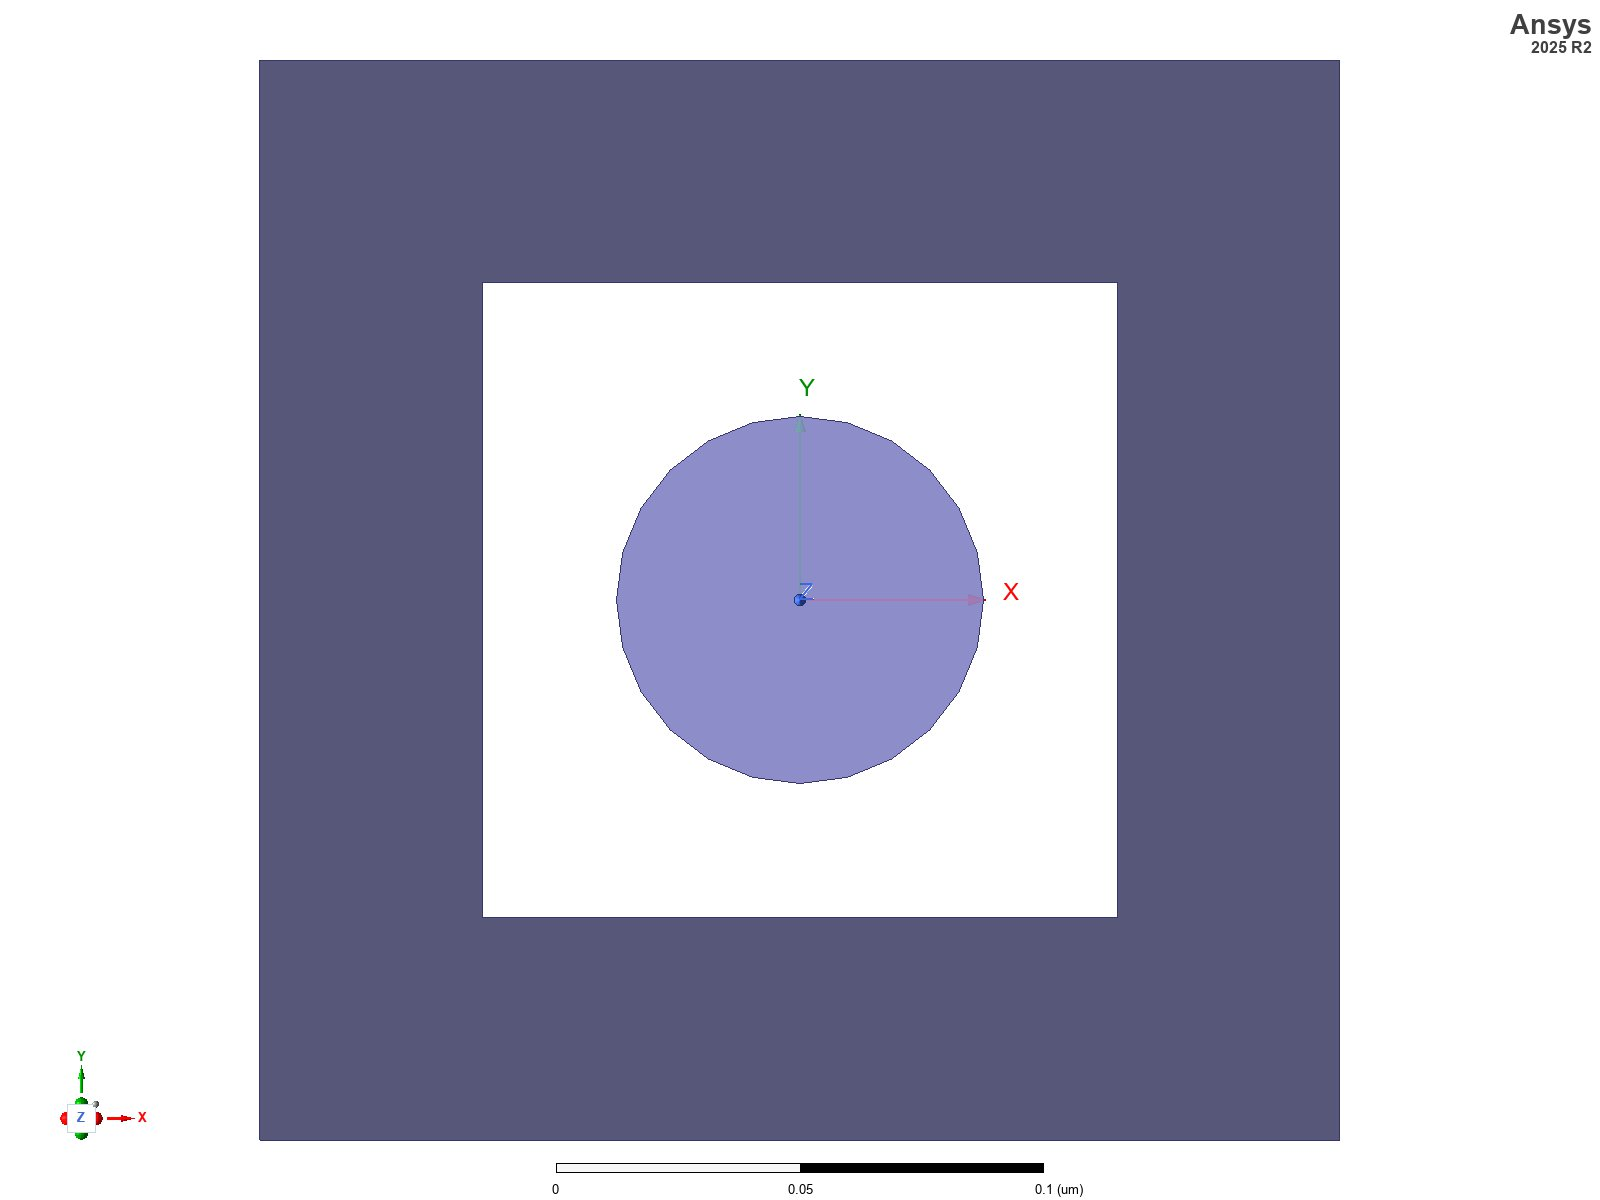
\includegraphics[width=.94\linewidth,height=.72\textheight,keepaspectratio]{assets/hfss/example_04.jpg}\par
{\small Optuna = Ray, F07. Target: 20\% over 1000--1040 nm.}\par{\scriptsize Top view exported from the verified HFSS project.}\end{frame}

\begin{frame}{Backup: HFSS geometry, example 5}\centering
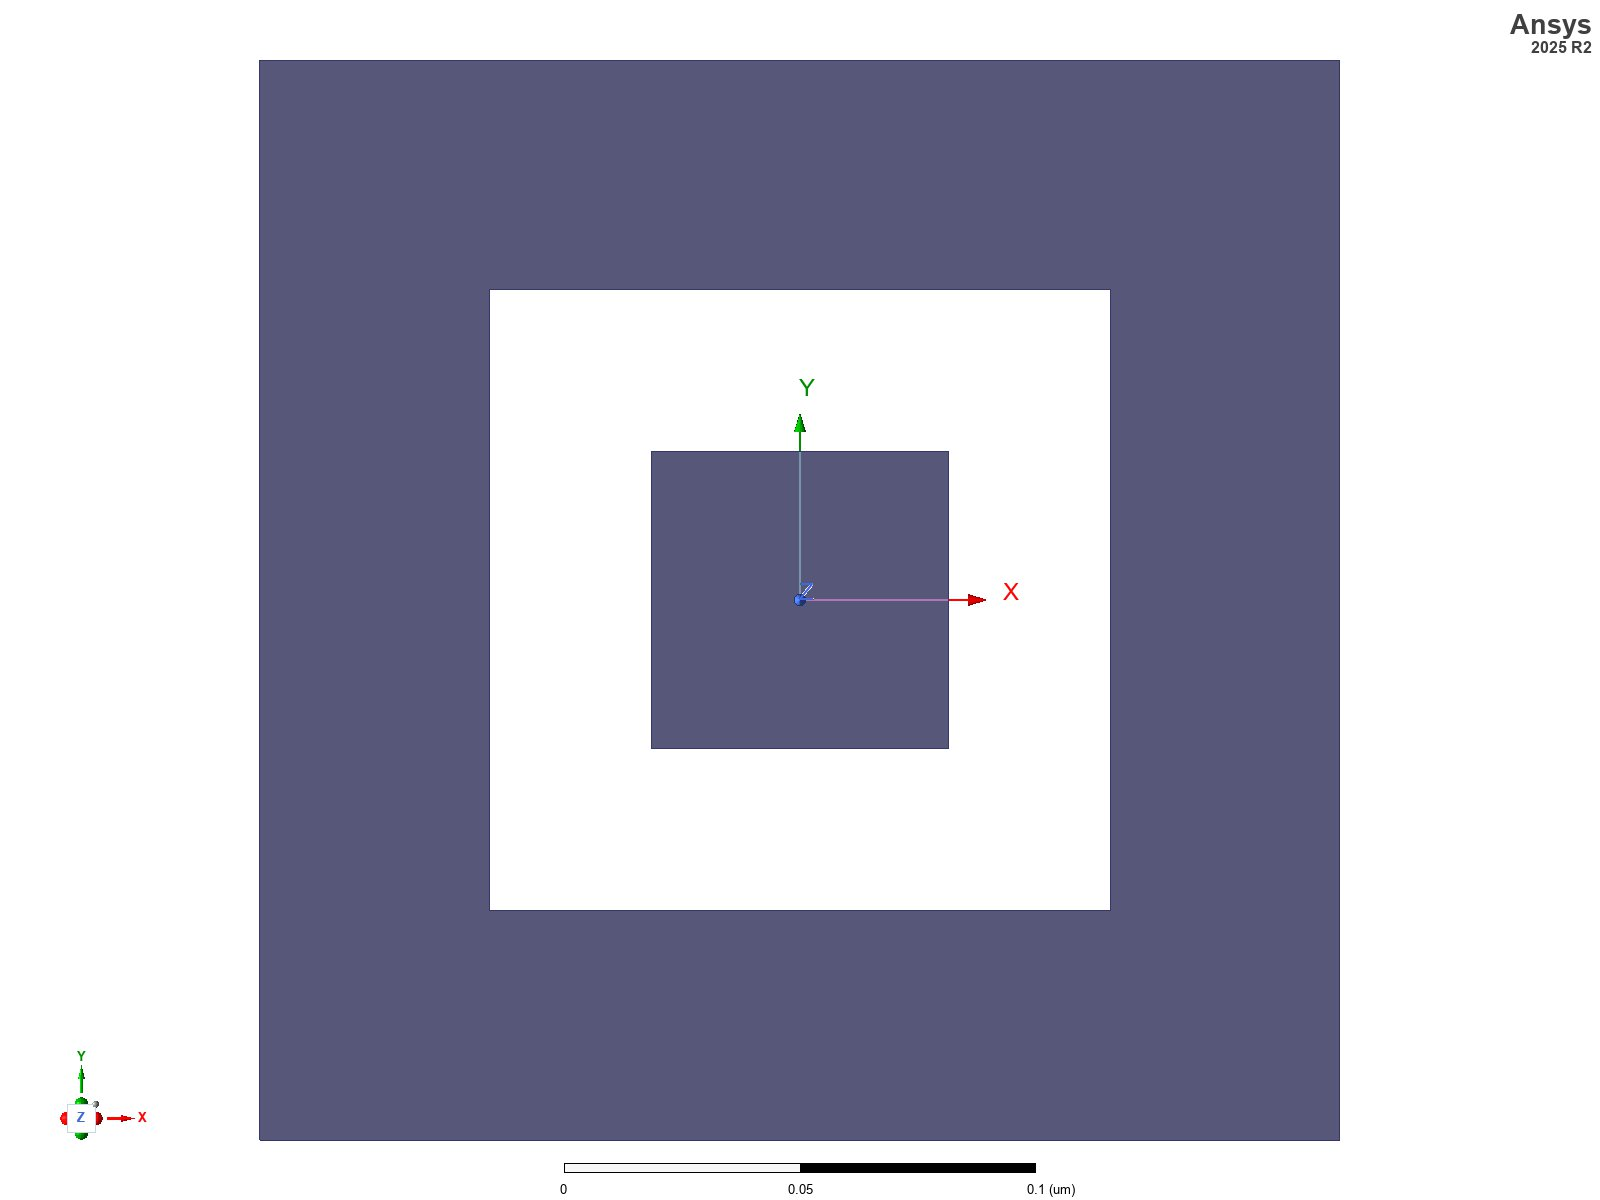
\includegraphics[width=.94\linewidth,height=.72\textheight,keepaspectratio]{assets/hfss/example_05.jpg}\par
{\small Optuna = Ray, F09. Target: 15\% over 1250--1300 nm.}\par{\scriptsize Top view exported from the verified HFSS project.}\end{frame}
\end{document}
